En primer lugar se tuvo que diseñar y construir un prototipo que respondiese a una serie de exigencias impuestas por el experimento. Por un lado este debía de ser capaz de albergar de manera segura  un bunch de 35 fibras centelleadoras, el cual se encontraría totalmente sumergido en una solución de agua tritiada estanca. Este prototipo debía de ser capaz de comunicar los extremos del bunch con contadores de fotones, los cuales deben estar aislados del agua tritiada, sin que existiese ningun tipo de fisura para asegurar que no existe peligro de fuga y, por tanto, de contaminación, nisiquiera por evaporación del agua. Por otro lado debía de sostener de forma segura el contador de fotones utilizado, en nuestro caso PMTs, para leer la señal recibida por estas fibras centelleadoras.

Con todas estas exigencias el materíal elegido para la construcción del prototipo fueron diversos elementos de fontanería de PVC. El motivo de este es su seguridad, ya que están especialmente diseñados para transportar y retener agua, su facilidad de manipulación ya que podemos realizar cortes con mucha rapidez, sencillez y eficacia además de existir muchas formas para diversos fines y, finalmente, su precio ya que se trata de un matería bastante económico. 

En concreto se utilizo un tubo de PVC de 2 metros de longitud y un diámetro interior de 15 mm, en el cual se practicaron una serie de cortes dando lugar a un conjunto de secciones que conformarían los 2 prototipos. Para unir cada una de estas secciones y dar forma al prototipo se utilizaron codos, típicamente utilizados en fontanería de PVC, cuyas uniones serían finalmente selladas con silicona. Finalmente el prototipo quedaría sujeto de forma segura sobre una estructura de metacrilato y acero. El aspecto final del prototipo puede verse reflejado en la figura 20.

\begin{figure}[hbtp]
\centering
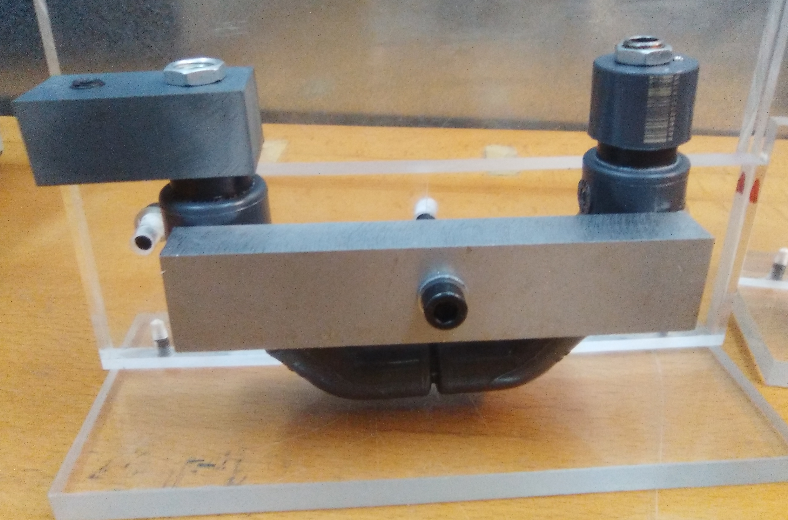
\includegraphics[scale=0.4]{Prototipo.png}
\caption{ Prototipo\label{prototipo}}
\end{figure}

Este prototipo presenta un volumen en su interior (el cual será rellenado por la soución radiactiva) de $39~\cm^3$, el cual se calculó y verificó con varios ensayos de llenado con agua destilada. También se verificó la permeabilidad del prototipo a partír de una estáncia de estos ensayos de 2 días. 

Podemos observar que se decidió realizar un prototipo con forma de U. Dado que el prototipo no se trasladará en ningun caso y, teniendo en cuenta que se verificó su permeabilidad, personalmente opino que esta es la forma más segura y que mejor se adapta a las exigencias del prototipo. Las dos oberturas superiores serán cerradas y selladas con tapones tipicamente utilizados en fontanería de PVC. Se eligieron tampones diferentes para cada extremo. Un primer tapón circular, acorde a la forma del tubo de PVC y un segundo tapón cuadrado, el cual nos facilitaría el proceso de llenado. Este segundo tapón dispone de dos orificios, uno de 8 mm por el que se realizará el proceso de llenado y otro de 1 mm por el que se purgará el aire durante el mismo proceso. Finalmente estos orificios se cerrarán con ayuda de dos tornillos de rosca envuletos en teflón. Estos tapones pueden verse reflejados en la imagen 20.

Además ambos extremos disponían también de un agujero de 9,8 mm de diámetro, tamaño justo para que por cada uno de estos pasara un extremo del bunch de fibras centelleadoras. En estos extremos se dispusieron dos arandelas, roscadas al aro que conformaba el extremo del bunch, según la imagen 5 (una arandela a cada extremo del tapon, parte interna y externa). De esta forma conseguíamos fijar perfectamente cada uno de los extremos del bunch al prototipo y comunicar el extremo de las fibras al exterior del prototipo para su correspondiente lectura con los contadores de fotones, PMTs en nuestro caso. 

En todo momento se utilizó silicona para sellar cualquier posible fisura del prototipo.

También podemos observar que se ha decidido realizar el giro de $180º$, correspondiente a la U, con ayuda de cuatro codos de $45º$ y no con dos codos de $90º$. Esto es debido a que, con giros progresivos, el bunch de fibras centelleadoras estarán sometidos a una tensión inferior y, por extensión, ofrecerán una mejor propagación de la señal.

Finalmente se utilizaron dos piezas, usualmente utilizadas en fontanería de PVC para comunicar tuberías de igual o diferente diámetro para sostener los PMTs en el prototipo. Debido al hecho de haber utilizado dos tapones distintos ahora necesitaremos dos piezas diferentes. Estas pueden verse en la figura 21.

\begin{figure}[hbtp]
\centering
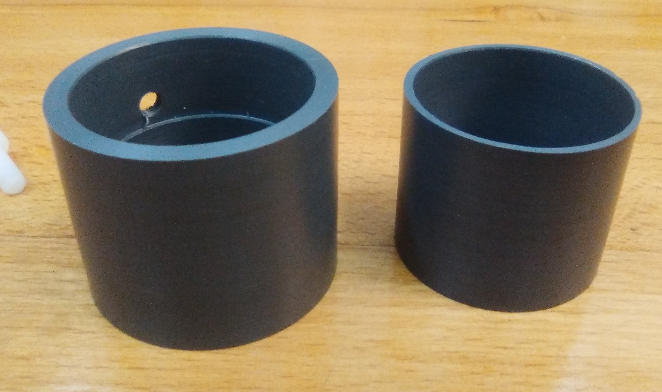
\includegraphics[scale=0.4]{Tapones.png}\\
\caption{ Piezas de sujeción de los PMTs\label{tapones}
}
\end{figure}

La primera pieza (correspondiente a la pieza derecha de esta figura), más pequeña, simplemente encajaba al tapón circular por un extremo y, por el otro, con un diámetro interior más grande para que cupiese y fijase, se disponía del PMT.

Para la segunda pieza encontramos un problema y es que no hay tuberías cuadradas, por lo que no encontramos ningun tipo de pieza como esta que ajustase a este tapón (tapón cuadrado del prototipo). En su lugar simplemente utilizamos una pieza para que encajase a la arandela que sobresalía del prototipo (utilizada para fijar el bunch de fibras) y por el otro extremo que encajase al PMT. Para mayor sujeción se utilizo en esta pieza un tornillo que unía esta a la plataforma de metacrilato. La disposición de estos en el prototipo y el tornillo que ayuda a la sujeción pueden verse reflejados en las imágenes de la figura 22.

\begin{figure}[htb]
\centering
{
%\subfloat[Espectro de emisión]
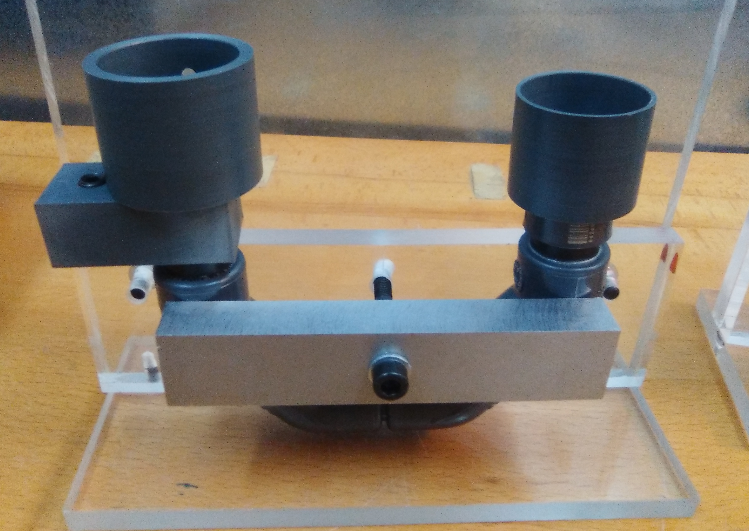
\includegraphics[scale=0.25]{Prototipodelantetapon.png} 
}
{
%\subfloat[Espectro de emisión]
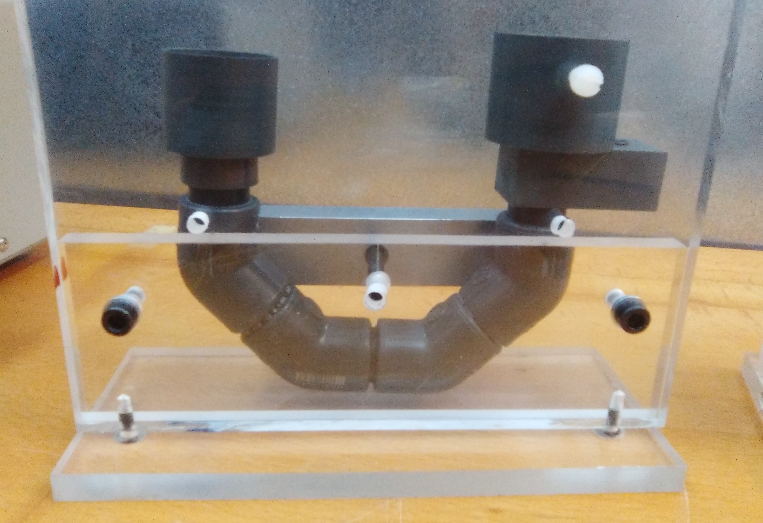
\includegraphics[scale=0.25]{PrototipoDetrastapon.png} 
}
\caption{Prototipo con piezas de sujeción \label{prototipotapones}}
\end{figure} 

Hay que tener en cuenta que el proceso de medida se desarrollará en el interior de una cámara oscura cuya única labor es la de protejer de la posible entrada de luz del exterior. En esta no habrá un control exhaustivo de la temperatura como ocurría con el sistema utilizado para la calibración de los SiPM. En su lugar únicamente activaremos el aire acondicionado en la sala para mantener una temperatura constante de aproximadamente $25ºC$ en todo momento.

Los PMTs empleados, R8520-ZB2771 y R8520-ZB2773 se alimentaron ambos a $-830$ V. A esta temperatura disponen de una ganancias de $G_1=1456178$ y $G_2=1921595$ y su eficiencia de fotodetección a $\lambda=430~nm$ es de $29.76\%$ y $28.66\%$ respectivamente. 
